\chapter{Methods}
\label{chapter_methods}
The target of this work is to implement an alternative solution to the existing source database of \ac{BIONDA}. However, before one can choose an alternative database or a development environment it is crucial to get a deeper understanding of the available data structure of Disease Ontology. Disease Ontology, as outlined in chapter \ref{chapter_results}, is a well maintained and frequently updated disease database. This is a necessary point to mention as the authenticity of such sensitive information requires monitoring by a public institution. All of the requirements (see table \ref{tab:evaluationmatrix}) are fulfilled, which allows one to take a deeper look into the available data structure. Disease Ontology references a public repository at Github. This specific repository is monthly updated, which can be regarded as quite reasonable, taking into consideration that the possibility of new diseases being discovered is rather low. Each monthly update consists of an updated file (HumanDO.obo) containing all diseases and each previous versions of this file. As mentioned before it is relevant to analyze the structure of this file to find a repeating pattern. This is especially important to extract just the diseases and ignore everything else. This process will be further explained in detail in the next sections.

\section{Requirements of a Disease Database}
In order to determine which of the mentioned databases is best to be integrated into \ac{BIONDA}, specific criteria need to be defined. Later, these criteria will be weighted according to the importance to the project lead. Beginning with the first criteria it is necessary to increase the search results while searching with \ac{BIONDA}. To find a specific disease it is significant to have trivial names of a specific biomarker or disease. This could solve the problem of a disease being named differently by other groups of people. A medicine researcher would name a disease by its medical name which would restrict the usability of the database to other fields. Anyhow, \ac{BIONDA} should be usable for every person in general, which makes the use of trivial names the number one criteria. Furthermore the database should be updated frequently. This would ensure that the latest research of publications would be immediately displayed on \ac{BIONDA}, as the selected database is always up to date and thus new diseases are frequently added to the database. This would ensure that \ac{BIONDA} could become a more easy to use disease database for many people. In addition, the selected database should contain a large number of entries. To ensure that the database is accessible to everyone it is essential for it to be freely accessible. It is crucial to have an \ac{API} or a database dump in any format which allows the development team to download and parse the disease entities. In summary the criteria for the \ac{UniProt} replacement are the following ones.

\begin{itemize} 
\item Trivial names available 
\item Update frequency guaranteed 
\item \ac{API} available 
\item High number of entries 
\item Freely accessible
\item From public organization
\end{itemize}

In order to create an evaluation matrix the established criteria need to be weighted and ranked. The most important criterion will be free and open accessibility. In the best case, the database should be accessible to everyone. Closely followed by the use of trivial names. This is especially important to non-scientists, as the medical terms of the diseases are often only used in research fields. Furthermore, the number of entries in the database as well as the update frequency are also very important. A high number of disease terms is essential to make an accurate search possible. The update frequency is as important as the number of entries. A database that receives frequent updates and always stays up-to-date can provide an overview of many new publications through the many entries and thus shed light on areas of medicine that have already been researched intensely. Finally, the last criterion is a working or existing \ac{API}. A working API, is essential to automatically download and parse the database. However, this criterion is the least weighted, since it was clear from a previous search that all databases have a limit and thus the entire database could not be downloaded at once. It is important to note, that the Disease Ontology database does not offer an API but a dump of the complete disease database. The file format of the database is purely text based, which allows to choose a development environment that suits the knowledge of the development team. The weights of the criteria can be seen in the following table. 

\begin{table}[h]
\centering
\begin{tabular}{|l|c|}
\hline
\textbf{Criterion}   & \multicolumn{1}{l|}{\textbf{Weight}} \\ \hline
Number of entries    & x4                                   \\ \hline
Synonyms             & x5                                   \\ \hline
Freely accessible    & x6                                   \\ \hline
Public organization  & x6                                   \\ \hline
API (unlimited) & x3                                   \\ \hline
Update frequency     & x4                                   \\ \hline
\end{tabular}
\caption{Weights of Database Criteria}
\end{table}

\section{Software, Hardware and Programming Language}
When developing a software component it is important to decide which programming language should be used. As argued in the requirements specification of this project (see appendix \ref{Anhang_Pflichtenheft}, figure \ref{bionda_structure}) the decision depends on the current setup of \ac{BIONDA}. \ac{BIONDA} has been developed with typical web based technologies but the backend has been developed in Java \citep{Liguori_Liguori_2018} with a MySQL \citep{DuBois2014} database which holds more than just the diseases (see section \ref{methods_database}). After discussing this question with the project lead it was clear to use Java for this project. However, this project is not entirely attached to the infrastructure of \ac{BIONDA}. The hardware used in this project is purely personalized. The developed component runs on a \ac{JRE} which can be used on every personal computer. Therefore no special hardware is required to run the component. The main task of the project is to feed new diseases into the \ac{BIONDA} database, which makes it independent and not linked to the backend neither frontend. \\

Organizing this project accordingly to the development software cycle it is essential to split the tasks into smaller ones. Overall one can say that the development part of the project comprises a text parsing and a database modeling component, which are both crucial for the application. In the following sections both components and the used technologies are explained in detail.

\section{Regular Expression}
Beginning with the first component \enquote{text parsing} it is significant to get an overview of the source and the format of the file. The file does not follow a widely known format like XML or Markdown. However, it does follow a format specially created by the \ac{OBO} Foundry. The mission of \ac{OBO} is to develop \enquote{a family of interoperable ontologies that are both logically well-formed and scientifically accurate} \citep{do}. To achieve this collaborative work, it follows these four principles, such as: open use, collaborative development, common syntax. More importantly, the foundry is overseen by an operation committee and work groups consisting of researchers located worldwide. This is especially significant in order to assure  that the content of the delivered data is verified. 
\begin{figure}[H]
\centering
\begin{lstlisting}[]
format-version: 1.2
data-version: doid/releases/2019-05-13/doid-non-classified.obo
date: 13:05:2019 09:41
saved-by: lschriml
auto-generated-by: OBO-Edit 2.3.1
subsetdef: DO_AGR_slim "DO_AGR_slim"
subsetdef: DO_cancer_slim "DO_cancer_slim"
...
default-namespace: disease_ontology
remark: The Disease Ontology content is available via the Creative Commons 
Public Domain Dedication CC0 1.0 Universal license 
(https://creativecommons.org/publicdomain/zero/1.0/).
ontology: doid/doid-non-classified.obo
property_value: http://purl.org/dc/elements/1.1/title "Human Disease Ontology" xsd:string
\end{lstlisting}
\caption{First Lines of the Human.obo File}
Source: \citep{do}
\end{figure}
Now focusing on the content of the delivered file one can observe that the first lines define properties like ontology type, creation date, created by and other information which are quite irrelevant for the project. Nonetheless, after those first introductory lines the main content of the file begins, the diseases. These are defined inside a specific sequence of characters named “[Term]”. This sequence precedes the properties of the disease. However, one can see the possible properties of each disease. It shall also be noted that some properties are multi-value properties, meaning a disease may contain zero to many values of these very properties. 

\begin{table}[H]
\centering
\resizebox{\textwidth}{!}{%
\begin{tabular}{|l|l|l|}
\hline
\multicolumn{1}{|c|}{\textbf{Property}} & \multicolumn{1}{c|}{\textbf{Type}} & \multicolumn{1}{c|}{\textbf{Example}}                                                                                                                                                                                                                                                                                \\ \hline
ID                                      & single value                       & id: DOID:0001816                                                                                                                                                                                                                                                                                                     \\ \hline
Name                                    & single value                       & name: angiosarcoma                                                                                                                                                                                                                                                                                                   \\ \hline
\multirow{3}{*}{Alternative DOID}       & \multirow{3}{*}{multi value}       & \multirow{2}{*}{alt\_id: DOID:267}                                                                                                                                                                                                                                                                                   \\
                                        &                                    &                                                                                                                                                                                                                                                                                                                      \\ \cline{3-3} 
                                        &                                    & alt\_id: DOID:4508                                                                                                                                                                                                                                                                                                   \\ \hline
Definition                              & single value                       & \begin{tabular}[c]{@{}l@{}}def: "A vascular cancer that derives\_from the cells that\\
 line the walls of blood vessels or lymphatic vessels."\\ {[}
url:http://en.wikipedia.org/wiki/Hemangiosarcoma, \\ ...{]}\end{tabular} \\ \hline
\multirow{2}{*}{Belongs to subsets}     & \multirow{2}{*}{multi value}       & subset: DO\_AGR\_slim                                                                                                                                                                                                                                                                                                \\ \cline{3-3} 
                                        &                                    & subset: NCIthesaurus                                                                                                                                                                                                                                                                                                 \\ \hline
\multirow{2}{*}{Synonyms}               & \multirow{2}{*}{multi value}       & synonym: "acetylsalicylic acid allergy" EXACT {[}{]}                                                                                                                                                                                                                                                                 \\ \cline{3-3} 
                                        &                                    & synonym: "ASA allergy" EXACT {[}{]}                                                                                                                                                                                                                                                                                  \\ \hline
\multirow{2}{*}{Ontology references}    & \multirow{2}{*}{multi value}       & xref: ICD10CM:E88.9                                                                                                                                                                                                                                                                                                  \\ \cline{3-3} 
                                        &                                    & xref: ICD9CM:277.9                                                                                                                                                                                                                                                                                                   \\ \hline
\multirow{2}{*}{Parent diseases}        & \multirow{2}{*}{multi value}       & is\_a: DOID:712 ! refractory hematologic cancer                                                                                                                                                                                                                                                                      \\ \cline{3-3} 
                                        &                                    & is\_a: DOID:9538 ! multiple myeloma                                                                                                                                                                                                                                                                                  \\ \hline
Created by                              & single value                       & created\_by: snadendla                                                                                                                                                                                                                                                                                               \\ \hline
Creation date                           & single value                       & creation\_date: 2011-06-15T02:48:20Z                                                                                                                                                                                                                                                                                 \\ \hline
Obsolete                                & single value                       & is\_obsolete: true                                                                                                                                                                                                                                                                                                   \\ \hline
\end{tabular}
}
\caption{Overview of Disease Properties}
Source: \citep{do}
\label{Tab_Disease_Properties}
\end{table}

Some diseases may also miss some of these properties. To get a better overview of the raw input that needs to be processed and extracted see appendix \ref{Anhang_SnippetDiseases}. These disease properties are mostly self-explanatory but some of them need to be explained in detail. The alternative disease ontology ids reference ids of diseases that may link to a similar one. However, some of them may be obsolete and do not reference any diseases. A crucial property is e.g. the synonyms. Those are one of the key features that led to the decision to pick disease ontology as a source database. Because of that the users of \ac{BIONDA} get a higher probability to find a disease with a search term that may not be a professional research term. Finally, the parent diseases are essential for building a connection between all diseases. Those connections allow us to build a graph\footnote{In graph theory, a graph is a structure consisting of a set of objects in which some pairs of the objects are in some sense related. The objects are mostly called vertices and each connection of vertices is called an edge \citep{Trudeau1993}.} which meets the requirement to build a hierarchical structure of the diseases. \\

Knowing what type of data is delivered and what needs to be extracted one can decide which technology is right to extract the data. Of course there are a lot of possibilities but when working with data extraction or any kind of pattern matching\footnote{Pattern matching is the process of checking if a given sequence of characters exist. However, the match usually has to be exact: "either it will or will not be a match." \citep{Hopcroft2007}} the most used technology is called \ac{RegExp}. \ac{RegExp} is a subfield of theoretical informatics and describes a specific pattern by means of a string. This string follows a specific syntax and rules to build a matching algorithm. The most common use of \ac{RegExp} is a functionality in text editors. The search and replace functionality in each text editor uses \ac{RegExp} to find a specific pattern. In detail \ac{RegExp} consists of constants, resembling sets of strings and operator symbols, which define operations over these sets. The following definition of \ac{RegExp} can be found in many literature about formal language theory \citep{Hopcroft2007}. \\

Given a finite alphabet $\Sigma$ the following constants are defined as a regular expressions.

\begin{itemize}
\item{$\varnothing$ is an empty set}
\item{$\epsilon$ is an empty string}
\item{\textit{A} in $\Sigma$ defines a set containing only the character \textit{A}}
\end{itemize}

Now, given the regular expression \textit{B} and \textit{C} it is possible to produce different matching patterns by using the following operations. 

\begin{itemize}
\item{Concatenating: expression \textit{BC} takes every string in \textit{B} and \textit{C} and produces a matching pattern matching every combination of the elements in \textit{B} and \textit{C}.}
\item{Alternation: expression \textit{B | C} matches any element in \textit{B} or \textit{C} but ignores elements that are already in \textit{B}.}
\item{Kleene star: expression \textit{B*} matches the smallest superset\footnote{In mathematics, a set A is a subset of a set B, or equivalently B is a superset of A, if A is contained in B. \citep{Hopcroft2007}} of \textit{B}, which contains an empty string, too.}
\end{itemize}

However, those basics are only a tiny portion of the functionality of \ac{RegExp}. The full explanation would exceed the scope of this work. For this very reason it is important to focus on the regular expression that extracts the diseases from the delivered file.\\

\begin{figure}[H]
\centering
\begin{lstlisting}[xleftmargin=0.24\textwidth, xrightmargin=0.22\textwidth]
\Q[Term]\E((?:(?!\Q[Term]\E|\Q[Typedef]\E)[\s\S])*)
\end{lstlisting}
\caption{Regular Expression for Diseases}
\end{figure}

In principle, this regular expression searches for every string containing the tokens \textit{[Term]} until another sequence of these characters is found. In this case, every string between those sequences will be matched and extracted. This assures that some tokens, defining the properties and begin with \textit{[Typedef]}, are not matched (see appendix \ref{Anhang_PatterMatching}). This is secured by creating groups inside the expression, which have to fulfill both criteria. In detail the expression applies this matching algorithm, which is a naive representation of \ac{RegExp}.

\begin{algorithm}[H]
\caption{Matching Algorithm}
\begin{algorithmic}[1]
\Require $string\_of\_diseases := S$
\State Initialize $ matched\_groups$
\ForEach {$line \in S$}
\State Initialize $ group $
\If {$\text{[Term]} = line$}
	\If {$\text{[Term]} \neq line + 1$}
    	\State $group \gets line + 1$
	\EndIf
\EndIf
\If {$line + 1$ empty}
	\If {$\text{[Term]} = line + 2$}
    	\State $matched\_groups \gets group$
	\EndIf
\EndIf
\EndFor
\Return $matched\_groups$
\end{algorithmic}
\end{algorithm}

At this point all diseases are extracted and ready to be inserted into the database. In the following section the disease insertion will be discussed in detail.


\section{Database Implementation}
\label{methods_database}
When building an application it is significant to choose a database architecture where all data is saved. However, \ac{BIONDA} already has an existing infrastructure (see figure \ref{bionda_structure}) and a database where all relevant data is stored. This makes the decision, which database architecture to choose, obsolete. This work focuses on the modification of the current database scheme, which is built on top of a MySQL server. In appendix \ref{Anhang_ER} the entity relationship model describes which new tables and relationships are added to the database. Especially the modifications on the existing disease table are displayed.

\begin{figure}[H]
\centering
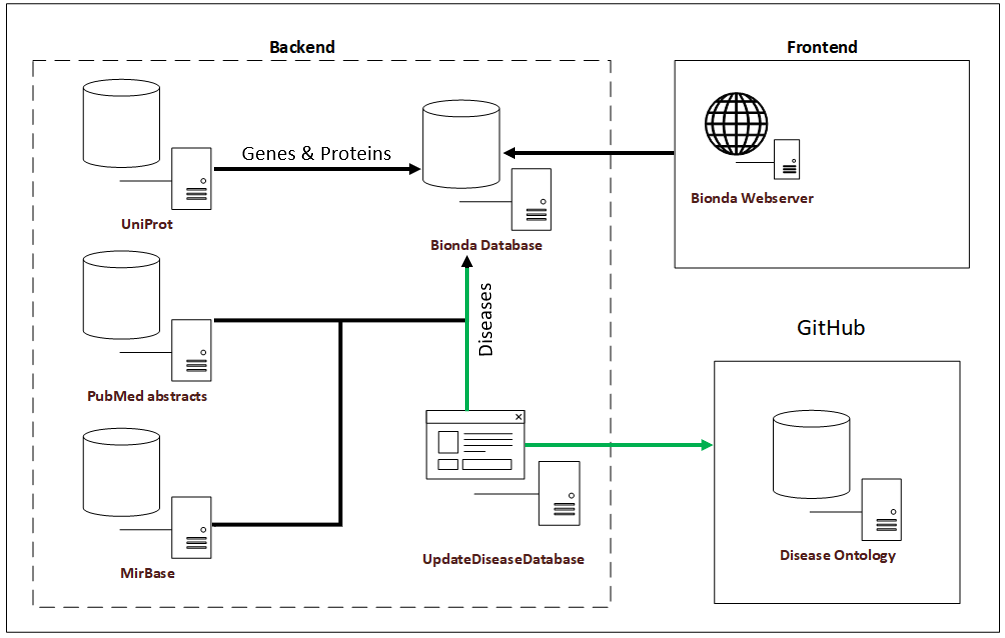
\includegraphics[scale=0.4]{bilder/Sollkonzept.png}
\caption{BIONDA Infrastructure}
\label{bionda_structure}
\end{figure}

When inserting the diseases into the database it is of great importance to consider the following two requirements:  Building relationships between the diseases and its multi-valued properties and creating the hierarchical data structure of the parent-child-relationships of these diseases. The relationships are crucial to guarantee the consistency of the database. In order to achieve this, the concept of foreign keys is applied on all newly-added and modified tables of the database. This makes sure that all database records are accordingly updated, in case of a modification or deletion. In order to solve the secondly-mentioned case, a typical relational database is not the best choice while working with graph-based data. Instead, the use of a graph-based database would be a better choice in this case. However, as explained in chapter \ref{chapter_results} the overall amount of diseases is 11,684 with 9,357 connections (edges) between those diseases. This number is more than feasible with a relational database. In order to build a graph from these connections, indexes and optimized queries make it possible to get a result in milliseconds. \\

This update mechanism is directly tied to the database. The whole workflow is developed in Java and a Java-MySQL-Connector to establish, add and update records of \ac{BIONDA}s database. In this very case a Java class has been implemented to offer all methods that are needed to handle the required operations (see appendix \ref{Anhang_Klassendiagramm}).

\section{Maintenance}
Now that there is an understanding of both components, it is of special interest to outline the maintenance of this application. Maintaining an application can be solved in several ways. Yet in the case of this specific one, it will consist of logging error messages, handling the case if the update process has been interrupted, modifying the applications behavior without source code changes and the implementation of additional methods, which output statistics of the parsed data of the disease ontology. All of this would happen during the update process of the database. Logging is an essential part of an application, especially with applications that are mostly working as a background process. As this is the case, logging is responsible for writing any errors or debug messages to a file on the current working directory. This includes any connection errors to the database or insertion of diseases. Downloading the disease ontology archive and possible permission errors are also written to the file. Each error is documented and corresponds to an error code, which can be referred to by the attached list of errors in appendix \ref{Anhang_ErrorList}.\\

Another case that can occur is an unexpected interruption of the update process. This could have several reasons. The best way to avoid any of these possible error states is to firstly, repeat the download process of the disease ontology archive if it gets interrupted. This may increase the overall runtime by several minutes due to the size of the archive. However, because time is not a constraint, it is reasonable to take this overhead if required. Secondly, the insertion of diseases into the databases can get interrupted, too. This could as well have many reasons, starting from a simple insertion error to a mysql timeout. A timeout could occur due to the fact that the insertion of nearly 12,000 diseases may take a while. Depending on the configuration of the mysql server a timeout may occur. To avoid this issue, the application fetches a list of pre-available diseases from the database. This list is then used to compare which diseases are missing and which need to be inserted. This routine solves any case of missing diseases in the \ac{BIONDA} database, even if all are missing.\\

Another significant feature of an application is to allow the user to modify the behavior of the application without any source code changes. This is accomplished by adding a configuration file, which contains all properties that influence the application. The properties change the behavior of all major tasks of the application. As an example, it is possible to change the update interval to a more suitable value. This increases the possibilities of this application. In the following table all possible properties are listed.

\begin{table}[H]
\resizebox{\textwidth}{!}{%
\begin{tabular}{|l|l|l|}
\hline
\textbf{Property}                & \textbf{Value Type} & \textbf{Example}                                                                                                                                          \\ \hline
db.user.name                     & String              & db.user.name=root                                                                                                                                         \\ \hline
db.user.password                 & String              & db.user.password=xxxx                                                                                                                                     \\ \hline
db.url                           & String              & \begin{tabular}[c]{@{}l@{}}db.url=jdbc:mysql://localhost:3306/bionda?\\ autoReconnect=true\\ \&useSSL=false\\ \&allowPublicKeyRetrieval=true\end{tabular} \\ \hline
repository.download.buffer\_size & Integer             & repository.download.buffer\_size=8192                                                                                                                     \\ \hline
repository.download.timeout      & Integer             & repository.download.timeout=1500000                                                                                                                       \\ \hline
repository.ontology.file\_name   & String              & repository.ontology.file\_name=HumanDO.obo                                                                                                                \\ \hline
repository.save\_path            & String              & repository.save\_path=user.home                                                                                                                           \\ \hline
repository.url                   & String              & \begin{tabular}[c]{@{}l@{}}repository.url=https://github.com/Disease\\ Ontology/HumanDiseaseOntology/archive/master.zip\end{tabular}                      \\ \hline
disease.update.interval          & Integer             & disease.update.interval=30                                                                                                                                \\ \hline
\end{tabular}%
}
\caption{Configuration Properties}
\label{tab:config}
\end{table}

Lastly, a few methods are implemented as part of the utility class (see appendix \ref{Anhang_Klassendiagramm}), offering a look inside the data. Especially, the diseases are further inspected in order to have a look at how many diseases have parents, which diseases have synonyms and how many ontology references they contain. It is also important to note that a function is implemented to get all obsolete diseases, which will be important for data science\footnote{\enquote{Data science is a multi-disciplinary field that uses scientific methods, processes, algorithms and systems to extract knowledge and insights from structured and unstructured data.}\citep{datascience}} purposes. In chapter \ref{chapter_results} the mentioned statistics will be further explained in detail. 
